\documentclass[a4paper,12pt]{article}

\usepackage{fontenc}
\usepackage[russian]{babel}
\usepackage[cp1251, utf8]{inputenc}
\usepackage{movie15}
\usepackage{graphicx}
\usepackage{amssymb, amsfonts, amsmath, indentfirst, enumerate, cite }
\usepackage{geometry}
\usepackage{hyperref}
%\graphicxpath{{//}}%путь к папке с картинками

\geometry{left=2cm}
\geometry{right=1.5cm}
\geometry{top=1cm}
\geometry{bottom=2cm}

\begin{document}
\begin{titlepage}
\begin{center}

\includegraphics[width=0.2\textwidth]{university_logo.jpg}
\end{center}

\begin{center}
\LARGE
Федеральное государственное бюджетное образовательное 
учреждение высшего образования "Московский автомобильно-дорожный 
государственный технический университет(МАДИ)"\\

\vspace{2cm}
Факультет "Автомобильного транспорта"\\
Кафедра "Высшая математика"\\


\vspace{2cm}
Курсовая работа по дисциплине\\
"Прикладное программирование и пакеты программ"\\
\end{center}

\vfill
\begin{flushright}
    
Выполнил:\\
Чарыков Д.В.\\
Группа 1бПМ1\\
Подпись\\
\vspace{1cm}
Принял\\
Доткулова А.С.\\
\vspace{1cm}
Подпись
\end{flushright}
\end{titlepage}
\tableofcontents
\newpage
\section*{Входные данные}
Видеоряд с камеры iVideonCute2 во временном промежутке 14:00 - 15:00 06.07.22
(День, хорошее освещение, без осадков, 2 битых файла)\\
Система мониторинга динамики транспортных потоков на базе метода виртуальных детектеров
- "ViDeS" / System for monitoring the dynamics of traffic flows based on
the method of virtual detectors - "ViDeS" (Virtual Detectors System)
\addcontentsline{toc}{section}{Входные данные}


\section*{Настройка детектеров}
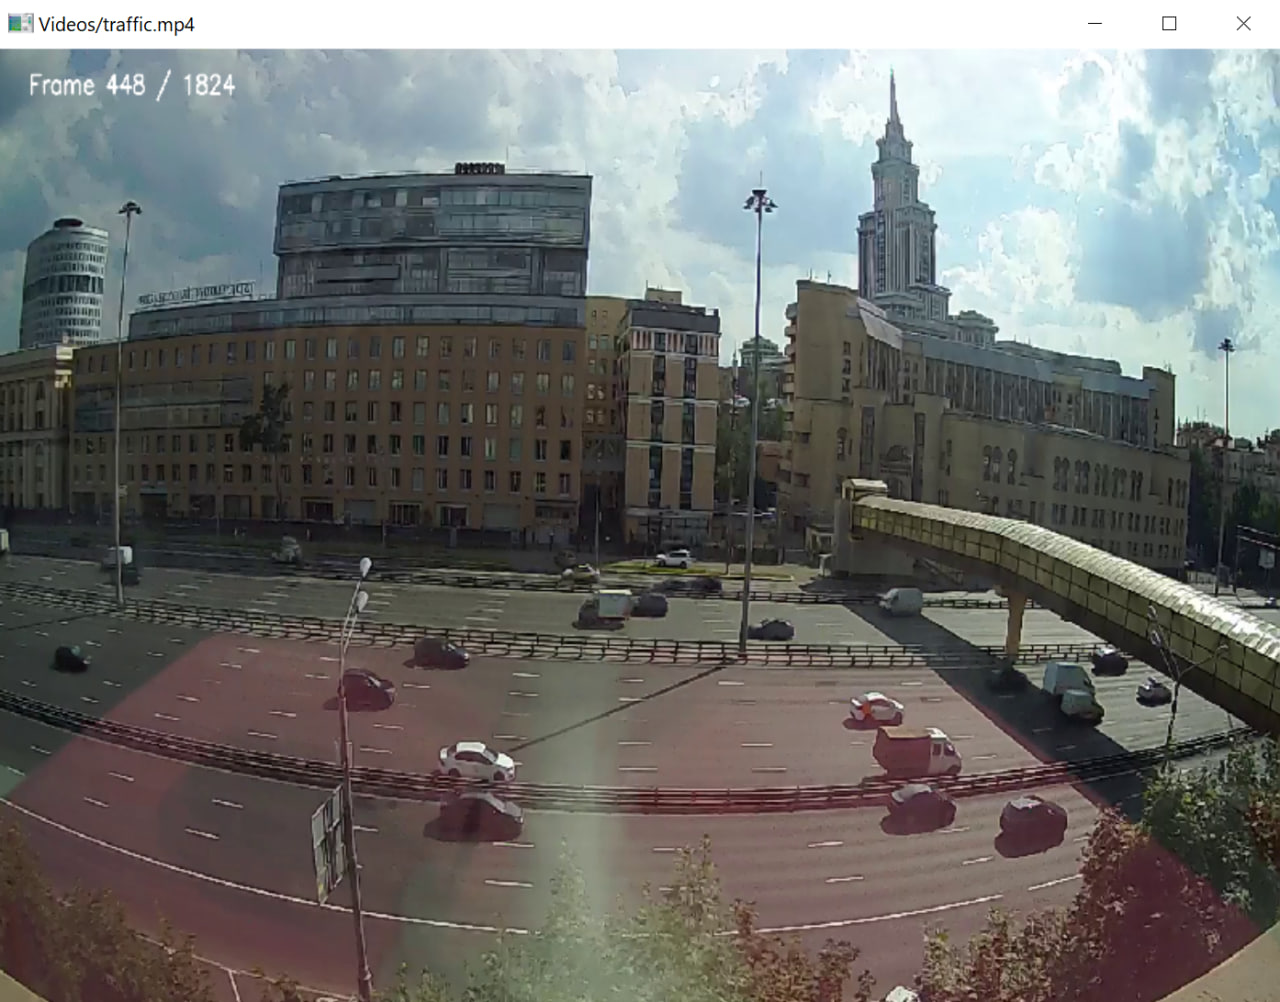
\includegraphics[width=0.8\textwidth]{detector_settings.jpg}
\begin{center}
Подбираем оптимальные данные для детектеров
\end{center}
\begin{enumerate}
    \item detector height: 20
    \item detector width: 50
    \item activation avg color delta 1.75
    \item frames unite: 10
\end{enumerate}
\begin{center}
При подобных параметрах датчиков мы имеем минимальную погрешность
\end{center}
Смотрим изменения цвета на детекторе это количество говорит нам сколько машин проехало
\begin{center}
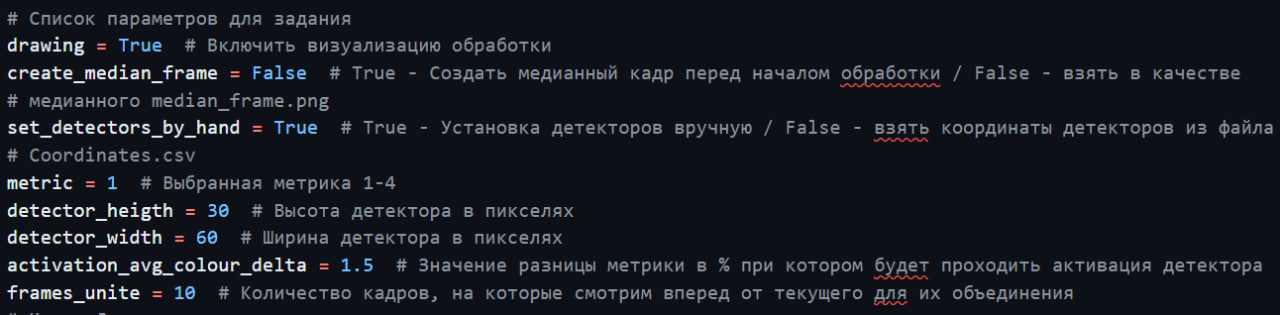
\includegraphics[width=0.9\textwidth]{detector_code.jpg}
\end{center}
\addcontentsline{toc}{section}{Настройка детектеров}


\newpage
\section*{Запуск "ViDeS"}
Для обработки видео, записанные в 30 кадров/сек, будем использовать "ViDeS"\\
Устанавливаем детекторы, примерно по 30 штук на каждую полосу, всего 89 штук
\begin{center}
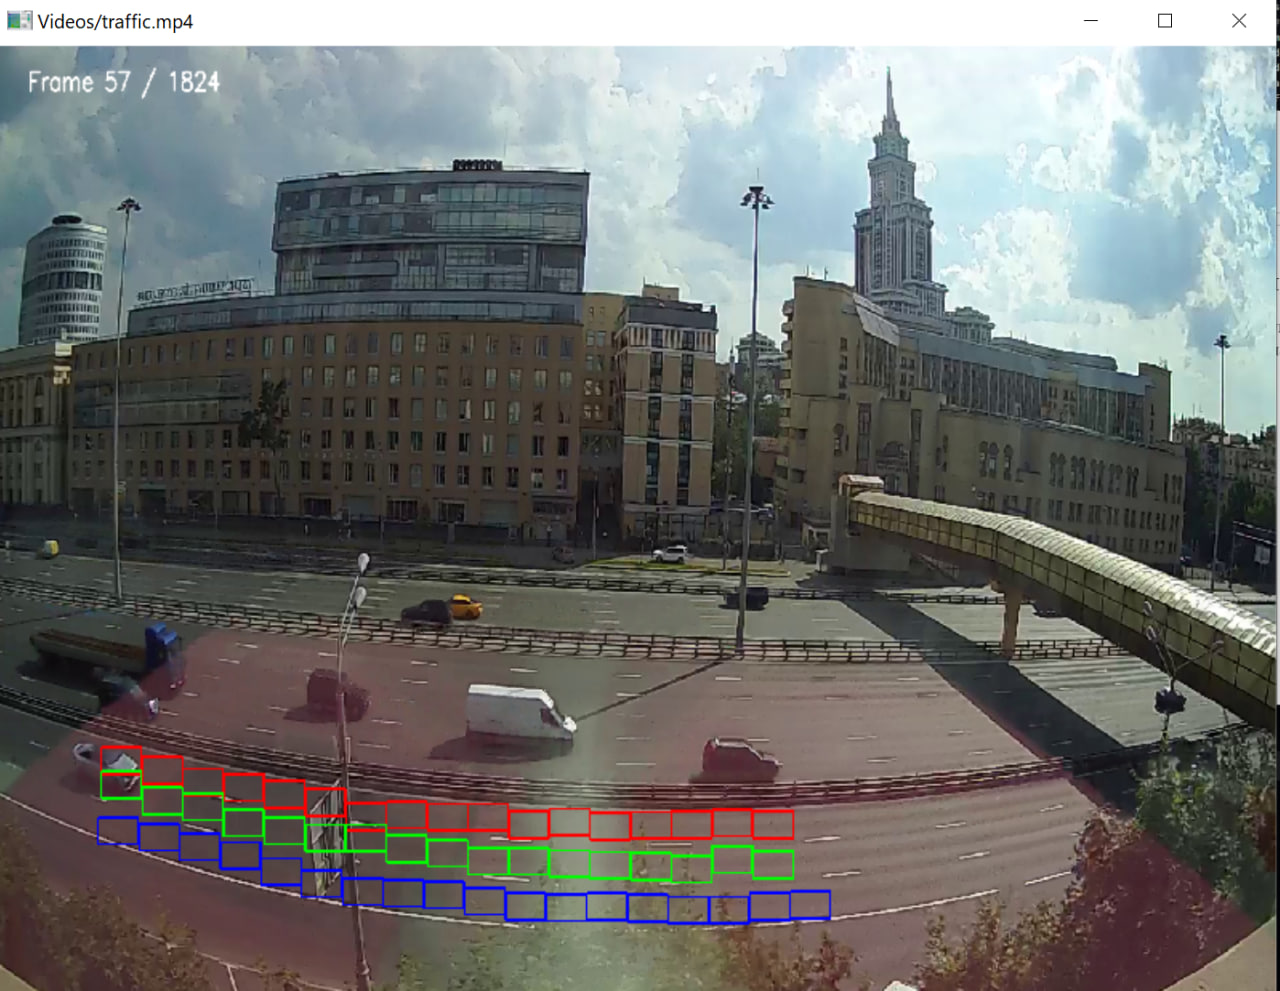
\includegraphics[width=0.9\textwidth]{vides_30_detectors.jpg}
\end{center}
После завершения программы, получаем .csv файлы с заполненными данными
Пример данных, содержащиеся в MetricValues.csv
\begin{center}
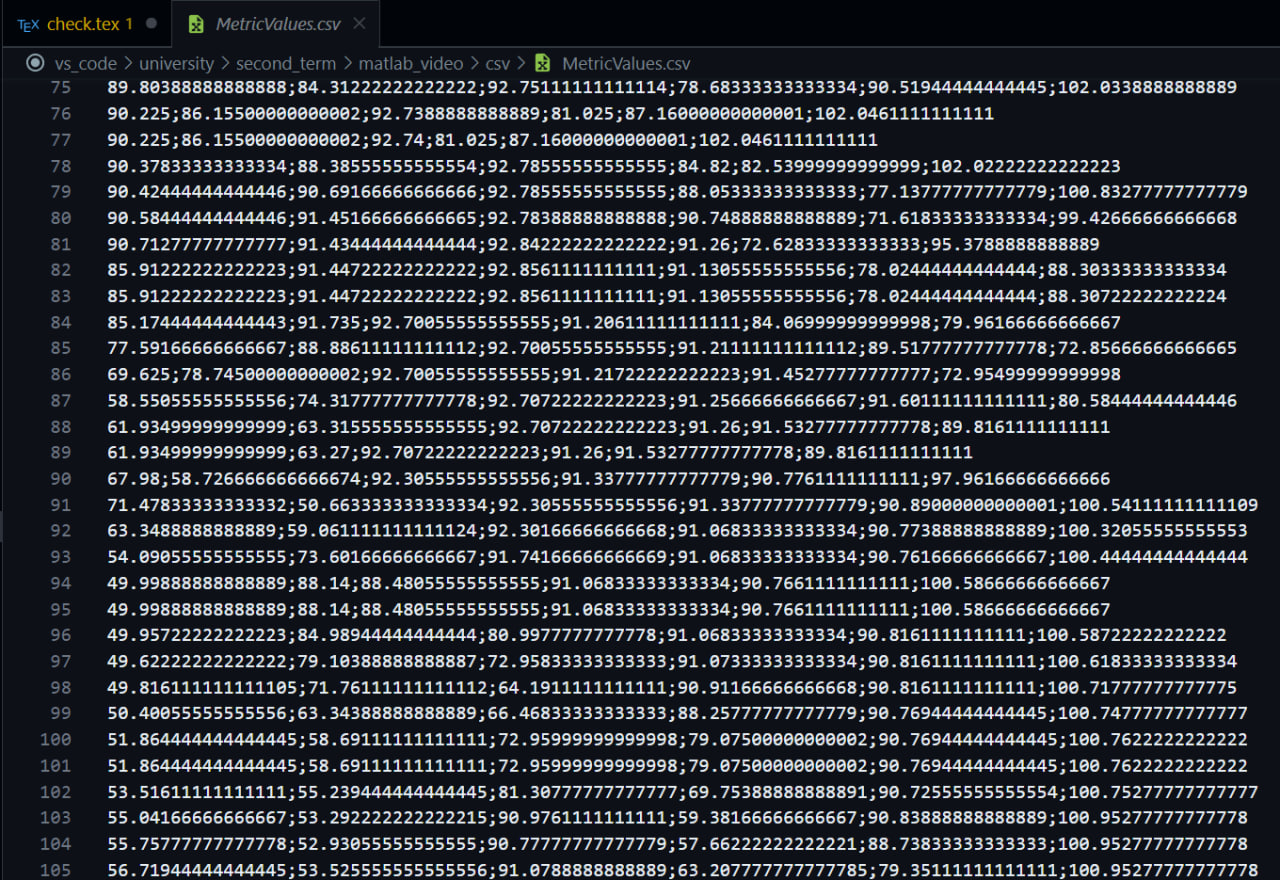
\includegraphics[width=0.9\textwidth]{vides_data.jpg}
\end{center}
\addcontentsline{toc}{section}{Запуск ViDeS}


\newpage
\section*{Построение гистограммы длин автомобилей}

Построили график, который показывает, сколько кадров машина находилась на детекторе\\
Благодоря этому мы может отследить скорость машины и всего потока в целом
\begin{center}
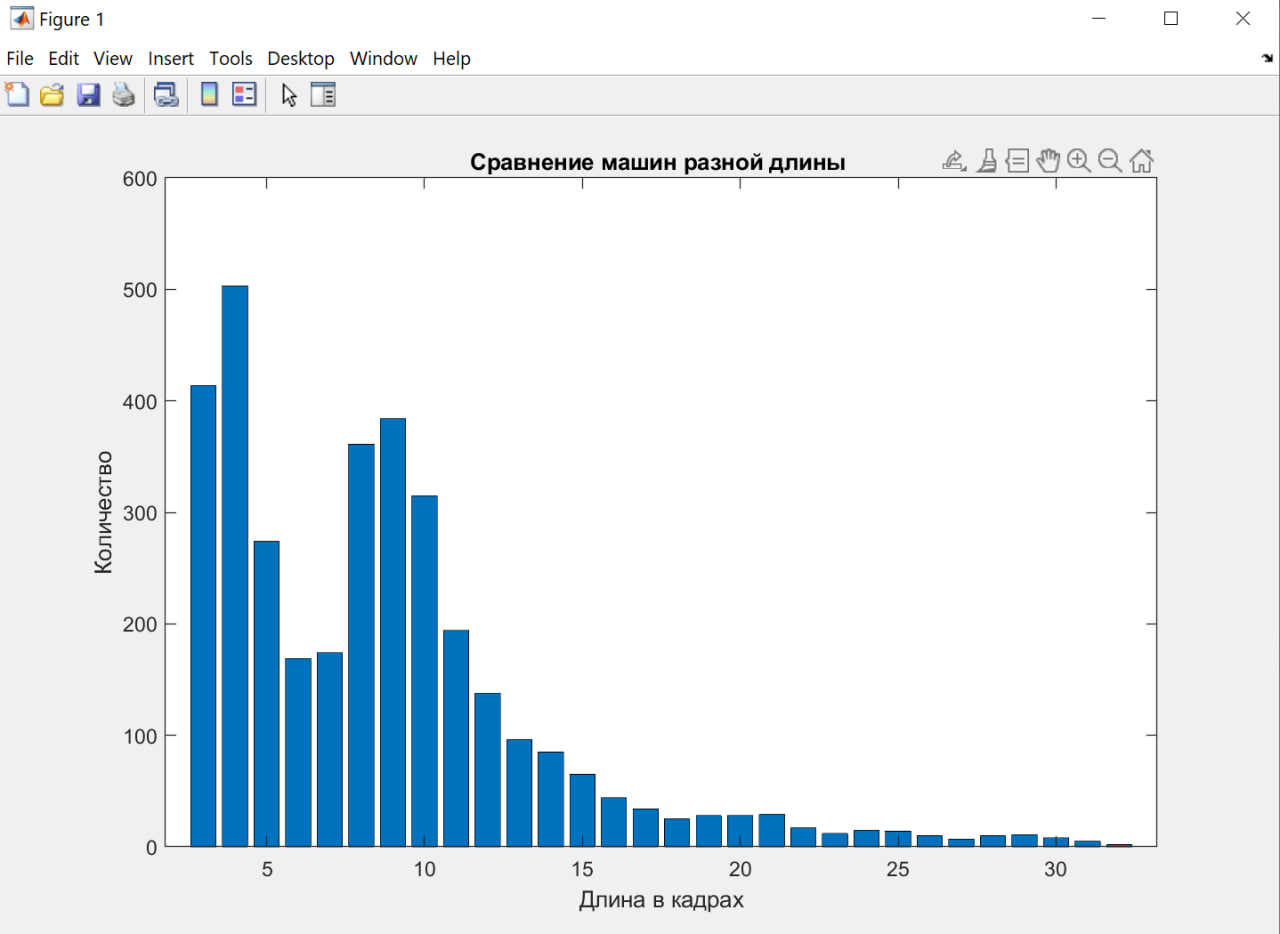
\includegraphics[width=0.9\textwidth]{histogram.jpg}
\end{center}
\addcontentsline{toc}{section}{Построение гистограммы длин автомобилей}


\section*{Построение графиков среднего цвета}
\addcontentsline{toc}{section}{Построение графиков среднего цвета}
\newpage
\section*{Построение бинаризированных графиков}
\addcontentsline{toc}{section}{Построение бинаризированных графиков}
\newpage
\section*{Построение совмещенных графиков}
\addcontentsline{toc}{section}{Построение совмещенных графиков}
\newpage
\section*{Вывод}
В результате проделанной работы удалось выяснить принциип работы детекторов, а также их точность.
При помощи ручной и автоматической оценки мы смогли оценить точно детекторов.
Построенные гистограммы длин автомобилей помогают оценить скороть транспортных средств,
А бинаризированные и совмещенные графики показывают плотность траффика.
Благодоря этим данным мы может проектировать будущие потоки, и избегать пробок
\addcontentsline{toc}{section}{Вывод}
\newpage
\end{document}
